% =====================================================================
%  Two Determinations Are Better Than One
%
%  This paper is self-contained.  External citations are to the mass
%  spectrometry, cheminformatics, and statistics literature only.
%  All numbers reported are measurements taken from the 58 CASMI 2022
%  priority challenges resolvable in the 17 mzML files held locally.
%  Nothing is simulated.
% =====================================================================
\documentclass[11pt,a4paper]{article}
\usepackage[utf8]{inputenc}
\usepackage[T1]{fontenc}
\usepackage{amsmath,amssymb,amsfonts,amsthm}
\usepackage{mathtools}
\usepackage[margin=1in]{geometry}
\usepackage{graphicx}
\usepackage{booktabs}
\usepackage{array}
\usepackage{enumitem}
\usepackage{lmodern}
\usepackage[protrusion=true,expansion=false]{microtype}
\usepackage[numbers,sort&compress]{natbib}
\usepackage[colorlinks=true,linkcolor=blue,citecolor=blue,urlcolor=blue]{hyperref}
\usepackage[capitalise,nameinlink]{cleveref}

\newtheorem{theorem}{Theorem}[section]
\newtheorem{lemma}[theorem]{Lemma}
\newtheorem{corollary}[theorem]{Corollary}
\newtheorem{proposition}[theorem]{Proposition}
\theoremstyle{definition}
\newtheorem{definition}[theorem]{Definition}
\newtheorem{axiom}[theorem]{Axiom}
\newtheorem{assumption}[theorem]{Assumption}
\newtheorem{construction}[theorem]{Construction}
\newtheorem{example}[theorem]{Example}
\theoremstyle{remark}
\newtheorem{remark}[theorem]{Remark}

\newcommand{\Dmass}{\mathcal{D}_{\mathrm{m}}}
\newcommand{\Dcon}{\mathcal{D}_{\mathrm{c}}}
\newcommand{\con}{\kappa}
\newcommand{\Fl}{\mathcal{F}}
\newcommand{\ppm}{\mathrm{ppm}}
\newcommand{\declineword}{\textsc{decline}}
\newcommand{\licenseword}{\textsc{license}}

\title{Two Determinations Are Better Than One:\\
Fragment Contact as Evidence Independent of Exact Mass,\\
and the Case for Declining to Answer}

\author{Kundai Farai Sachikonye\\
\texttt{kundai.sachikonye@wzw.tum.de}}
\date{\today}

\begin{document}
\maketitle

\begin{abstract}
Exact mass does not identify a small molecule. On 58 CASMI 2022 priority
challenges recovered from seventeen locally held Q~Exactive HF files, the number
of CHNOPS formulas reproducing the measured precursor within the instrument's
8~ppm window has median 183 and maximum 4500, and in \emph{zero} of the 58 cases
is that number one. Any method that answers from mass alone is therefore choosing
among survivors on grounds it has not stated. We introduce a second determination
that does not consult the precursor: \emph{fragment contact}, the
intensity-weighted fraction of the observed fragment ladder that a candidate
formula explains as its own subformulas. Contact is measured on the three stepped
collision energies (35/45/65~eV) as separate evidence channels rather than an
average. We then license an answer only where contact clears an absolute floor
and beats its nearest genuine rival by a margin; otherwise the method declines.
Three controls establish that contact carries information mass does not. A
same-mass decoy test separates the top candidate from its mass-indistinguishable
rivals by $+0.106$ in 53 of 58 challenges. A shuffle control scoring each
candidate on another compound's fragments drops its contact by a quarter,
$0.469 \to 0.342$.
Contact is not a size artefact: across 4684 candidate--fragment pairs the
correlation with heavy-atom count is $r = +0.058$. Under the floor, 5 of 58
challenges are licensed and 53 are declined --- a low yield we report as the
result rather than tune away, because a contest that grades a wrong answer and a
blank identically rewards exactly the confidence a method cannot honestly supply.
We state two defects plainly: one of the five licensed answers has its margin
carried by a chemical prior rather than by evidence, and no answer key was
available, so nothing here is graded against truth.
\end{abstract}

\tableofcontents

% =====================================================================
\section{Introduction}
% =====================================================================

\subsection{The problem is not sensitivity}

Untargeted liquid chromatography--tandem mass spectrometry routinely acquires
tens of thousands of high-quality MS/MS spectra per study, of which the large
majority are never assigned a structure~\citep{dasilva2015illuminating,
blazenovic2018software}. The bottleneck is not detection. The instrument sees the
compound, measures its mass to a few parts per million, and fragments it. What is
missing is a defensible route from those measurements to a name.

The CASMI series was created to measure that route
honestly~\citep{schymanski2017critical}. The 2022 edition posed 500 compounds
deliberately absent from public spectral libraries, 250 of them designated
priority, and graded four separate categories: the adduct, the elemental formula,
the structure class, and the 2D structure. Grading the formula separately from the
structure is the design decision that makes the contest useful here, because it
isolates the step at which most pipelines quietly guess.

\subsection{Mass alone is not a determination}

The reason it is a guess is arithmetic, and it has been known for two
decades~\citep{kind2006metabolomic,kind2007seven}. The set of elemental
compositions consistent with a measured $m/z$ grows superlinearly with mass and
does not collapse to a singleton at any tolerance an Orbitrap can
deliver~\citep{makarov2000electrostatic}. We restate this as a measurement on the
present data in \Cref{sec:degeneracy}: at 8~ppm the median challenge admits 183
formulas, and tightening the window to 1~ppm --- an accuracy the instrument does
not have --- still leaves the typical challenge with more than one survivor.

The standard response is to rank the survivors: by mass error, by isotope
pattern, by heuristic plausibility, by a library score, or by a learned
model~\citep{pluskal2012highly,duhrkop2019sirius,ruttkies2016metfrag}. Ranking is
not wrong, but it changes the question. A ranking always produces a first place.
It produces one when the evidence separates the candidates and it produces one
when the evidence does not, and nothing in the output distinguishes those two
situations. That indistinguishability is the defect this paper is about.

\subsection{What we propose}

We take two determinations of the same molecule and require them to agree.

\begin{itemize}[leftmargin=1.4em]
\item \textbf{$\Dmass$, the mass determination.} Every (adduct, CHNOPS formula)
pair reproducing the measured precursor within 8~ppm and surviving valence and
composition constraints. This is the standard construction and it is heavily
degenerate.
\item \textbf{$\Dcon$, the contact determination.} For each candidate, the
intensity-weighted fraction of the observed fragment ladder that is a subformula
of that candidate, computed on the fragment masses --- which $\Dmass$ never
consults.
\end{itemize}

The two determinations read disjoint parts of the measurement. $\Dmass$ sees one
number, the precursor. $\Dcon$ sees the fragment ladder and never the precursor.
Agreement between them is therefore evidential rather than tautological, and the
degree of agreement is a quantity we can measure and control.

\subsection{The decline}

We then do the thing that ranking cannot. We fix a floor $\beta$ on contact and a
floor $\mu$ on the margin over the nearest genuine rival, and we emit an answer
only where both are cleared. Otherwise the method returns \declineword{} and the
challenge is left blank.

This costs us. Under CASMI's scoring a blank earns nothing, and a method
declining 53 of 58 challenges will place poorly against one that answers all 58.
We report the low yield as the finding. The alternative --- lowering the floor
until the answer count looks respectable --- produces a submission whose entries
are indistinguishable in kind from the ones it declined, which is precisely the
state of affairs the floor exists to prevent. Selective prediction with an
explicit reject option is a well-posed problem with a known
theory~\citep{chow2008reject,herbei2006classification}; what is unusual in
metabolite identification is not the idea but the willingness to publish the
rejection rate.

\subsection{Contributions}

\begin{enumerate}[leftmargin=1.6em]
\item A measurement, on real contest data, that exact mass gives a unique formula
in \emph{0 of 58} challenges, with the full degeneracy distribution reported
uncapped (\Cref{sec:degeneracy}).
\item A contact determination computed over stepped collision energies held as
separate channels, with the algorithmic construction that makes it tractable
(\Cref{sec:contact}).
\item A licensing rule with an explicit decline, and its measured yield
(\Cref{sec:licensing}).
\item Three controls --- decoy, shuffle, and size --- establishing that contact
is independent of mass and is not an artefact of formula size
(\Cref{sec:validation}).
\item Two honestly stated defects, one internal to the method and one external to
it (\Cref{sec:defects}).
\end{enumerate}

% =====================================================================
\section{Data and instrument}
\label{sec:data}
% =====================================================================

\subsection{Provenance}

Seventeen mzML files (approximately 620~MB) were converted from Thermo raw format
by ProteoWizard 3.0.22040~\citep{chambers2012crossplatform} to indexedmzML
1.1.0~\citep{martens2011mzml}. The instrument is a Thermo Q~Exactive HF
(\texttt{MS:1002523}) operated under Xcalibur 2.8. Binary arrays are
zlib-compressed 64-bit floats. The files divide 8 positive-mode and 9
negative-mode acquisitions across five sample groups (M3--M7) on a
pentafluorophenyl column.

Fragmentation is HCD~\citep{olsen2007higher} at a stepped collision energy of
35.0, 45.0, and 65.0~eV. Every precursor is therefore fragmented three times in
consecutive scans. We verified this on the extracted set: the collision-energy
values encountered across all 1378 MS/MS scans are exactly $\{35.0, 45.0,
65.0\}$, with no other value present.

\subsection{Challenge recovery}

The priority challenge list (250 entries) and the challenge-81 erratum were read
directly from the distributed spreadsheets. Each challenge specifies a precursor
$m/z$, a retention time, and a source file. Matching each challenge against the
isolation windows of the local files with a tolerance of 0.01~Da on the isolation
target and 0.35~min on retention time recovers \textbf{58 of the 250 priority
challenges}, and all 58 are matched --- there is no challenge that falls in a
local file and fails to extract.

\begin{table}[!htbp]
\centering
\caption{Recovery of priority challenges from the seventeen local acquisitions.
Every challenge falling in a local file was recovered with its full
three-energy ladder intact.}
\label{tab:recovery}
\begin{tabular}{lr}
\toprule
Quantity & Value \\
\midrule
Priority challenges published            & 250 \\
Falling within the 17 local files        & 58 \\
Successfully extracted                   & 58 \\
MS/MS scans recovered                    & 1378 \\
Distinct collision energies              & 3 (35.0, 45.0, 65.0 eV) \\
Negative-mode scans                      & 842 \\
Positive-mode scans                      & 536 \\
Peaks per scan (min / median / max)       & 2 / 17 / 294 \\
\bottomrule
\end{tabular}
\end{table}

\begin{remark}
The 58 are not a curated easy subset. They are simply the challenges whose source
files were among the seventeen downloaded, and the download was constrained by
disk space rather than by any property of the compounds. The mass range spans
roughly $m/z$ 130 to 720 and both polarities.
\end{remark}

% =====================================================================
\section{The mass determination and its degeneracy}
\label{sec:degeneracy}
% =====================================================================

\subsection{Construction}

Let $z$ be the observed precursor $m/z$ in polarity $p$. For an adduct $a$ with
multiplicity $n_a$, added atoms $A_a$, removed atoms $R_a$ and charge sign
$s_a$, a neutral formula $F$ is mass-consistent when
\begin{equation}
\left| \frac{M(F)\,n_a + M(A_a) - M(R_a) - s_a m_e}{|s_a|} - z \right|
\;\le\; \frac{z \cdot \ppm_{\max}}{10^6},
\label{eq:d1}
\end{equation}
with $\ppm_{\max} = 8$ and $m_e$ the electron mass. Fourteen adducts are
considered: eight in positive mode ($[M+\mathrm{H}]^+$, $[M+\mathrm{Na}]^+$,
$[M+\mathrm{K}]^+$, $[M+\mathrm{NH_4}]^+$, $[M+\mathrm{H}-\mathrm{H_2O}]^+$,
$[M+\mathrm{H}-2\mathrm{H_2O}]^+$, $[2M+\mathrm{H}]^+$, $[2M+\mathrm{Na}]^+$) and
six in negative ($[M-\mathrm{H}]^-$, $[M+\mathrm{Cl}]^-$,
$[M+\mathrm{HCOO}]^-$, $[M+\mathrm{CH_3COO}]^-$,
$[M-\mathrm{H_2O}-\mathrm{H}]^-$, $[2M-\mathrm{H}]^-$).

Candidates are filtered by valence and composition constraints in the tradition
of Senior's rules and their modern heuristic
descendants~\citep{senior1951partitions,kind2007seven}: the ring-plus-double-bond
equivalent must lie in $[0,40]$ and satisfy the half-integer parity condition for
the ion's charge state; $\mathrm{H}/\mathrm{C} \in [0.1, 3.1]$;
$\mathrm{N}/\mathrm{C} \le 1.3$; $\mathrm{O}/\mathrm{C} \le 1.5$;
$\mathrm{P}/\mathrm{C} \le 0.35$; $\mathrm{S}/\mathrm{C} \le 0.35$; and absolute
caps $\mathrm{P} \le 4$, $\mathrm{S} \le 4$, $\mathrm{N} \le 12$,
$\mathrm{P}+\mathrm{S} \le 5$.

\begin{remark}[Why the absolute caps were necessary]
Ratio constraints alone do not bound heteroatom count at high carbon number. In an
early configuration without the absolute caps, formulas such as
$\mathrm{C}_{33}\mathrm{H}_{56}\mathrm{N}_2\mathrm{O}\mathrm{P}_2\mathrm{S}_5$
survived filtering: every ratio is satisfied, and no ratio notices that five
sulfurs and two phosphorus atoms on one skeleton describes nothing in a
metabolomics sample. The caps are stated here because they are a real
modelling commitment, not a tuning detail --- they encode the assumption that the
sample is biological.
\end{remark}

\subsection{The measurement}

\begin{table}[!htbp]
\centering
\caption{Degeneracy of the mass determination across the 58 challenges. Counts
are \emph{uncapped}: they are the full number of distinct formulas satisfying
\Cref{eq:d1} and the composition constraints, before any computational limit on
how many are subsequently scored.}
\label{tab:degeneracy}
\begin{tabular}{lr}
\toprule
Distinct formulas within 8~ppm & Value \\
\midrule
Minimum                                  & 4 \\
Median                                   & 183 \\
Mean                                     & 645 \\
Maximum                                  & 4500 \\
\midrule
Challenges with a \emph{unique} formula   & \textbf{0 of 58} \\
\bottomrule
\end{tabular}
\end{table}

\begin{proposition}[Mass does not determine formula on this data]
\label{prop:degeneracy}
On the 58 recovered challenges, the mass determination $\Dmass$ returns a
singleton in no case. Its median cardinality is 183 and its maximum is 4500.
\end{proposition}

\begin{proof}
By direct enumeration (\Cref{tab:degeneracy}). The construction is exhaustive over
the fourteen adducts and the CHNOPS composition space bounded by the constraints
of \Cref{sec:degeneracy}; no candidate satisfying \Cref{eq:d1} is discarded before
counting.
\end{proof}

\begin{remark}[A reporting hazard we fell into]
An intermediate implementation capped the number of candidates carried forward
for scoring at 120 for tractability. Reading the degeneracy off that stage
reports ``median 120, maximum 120'' --- a statistic about the cap, not about the
chemistry. Every degeneracy figure in this paper is taken before the cap. We
record the error because the capped number is the one a pipeline naturally
surfaces, and it understates the problem by a factor of nearly 40 at the tail.
\end{remark}

\subsection{Tightening the tolerance does not rescue it}

Because the degeneracy is driven by the density of the composition lattice rather
than by measurement noise, narrowing the mass window removes candidates slowly.
\Cref{fig:panel2} shows the measured candidate count as a function of tolerance
from 1 to 20~ppm across the mass range. The count falls roughly linearly in the
tolerance while the lattice density rises with mass, so at the upper end of the
range the curves do not approach one at any tolerance an Orbitrap delivers. This
is the empirical content of the claim that improved mass accuracy is not the
solution~\citep{kind2006metabolomic}.

% =====================================================================
\section{The contact determination}
\label{sec:contact}
% =====================================================================

\subsection{Definition}

\begin{definition}[Fragment ladder]
\label{def:ladder}
Fix a challenge with precursor $z$. For each collision energy $e \in \{35, 45,
65\}$, normalise every scan at that energy to its base peak and retain peaks at
relative intensity $\ge 0.01$. Merge across scans at $m/z$ resolution $10^{-4}$,
then collapse peaks within 8~mDa keeping the most intense member. The
\emph{ladder} $L$ is the resulting peak set restricted to $m/z < z - 0.5$,
truncated to the 60 most intense peaks. Each peak $f \in L$ carries a relative
intensity $r_f$ and the number $n_f \in \{1,2,3\}$ of energies at which it was
observed.
\end{definition}

The restriction $m/z < z - 0.5$ excludes the surviving precursor. This matters:
the precursor is trivially a subformula of itself, so including it awards every
candidate a large free contribution and compresses the differences the
determination exists to measure.

\begin{definition}[Contact]
\label{def:contact}
For a candidate neutral formula $F$ with adduct $a$, let $\mathrm{Sub}(F,a)$ be the
set of masses of ionised subformulas of $F$ --- formulas $G$ with $G_x \le F_x$
for every element $x$, adjusted for the adduct's charge carrier. Write $f
\rightsquigarrow F$ when some $G \in \mathrm{Sub}(F,a)$ matches $f$ within
$\max(12~\ppm, 4~\mathrm{mDa})$. The contact of $F$ is
\begin{equation}
\con(F) \;=\;
\frac{\displaystyle\sum_{f \in L,\; f \rightsquigarrow F} w_f}
     {\displaystyle\sum_{f \in L} w_f},
\qquad
w_f \;=\; r_f\bigl(1 + \tfrac{1}{2}(n_f - 1)\bigr).
\label{eq:contact}
\end{equation}
\end{definition}

\subsection{Why the three energies are kept separate}

The weight $w_f$ increases by 50\% for each additional collision energy at which
a peak appears. A peak surviving 35, 45 and 65~eV is worth twice a peak seen at
one energy alone. This is the only place the stepped-energy design enters, and it
is deliberate: averaging the three spectra into one, the more common treatment,
discards exactly the reproducibility information that distinguishes a real
fragment from a coeluting contaminant or a noise peak that happened to clear the
intensity threshold.

\Cref{fig:panel3} shows what the three channels actually contain on this data.
Precursor survival falls monotonically with energy while the intensity-weighted
mean fragment mass falls with it, so the three energies are not redundant
measurements of one spectrum --- they sample different depths of the
fragmentation cascade.

\subsection{The absolute floor on fragment tolerance}

The tolerance in \Cref{def:contact} is $\max(12~\ppm, 4~\mathrm{mDa})$ rather than
12~ppm alone. At $m/z\,91$ --- the tropylium region where many aromatic ladders
concentrate --- 12~ppm is $\pm 1.1$~mDa, which is tighter than the $m/z$
resolution at which the ladder is merged. A relative-only tolerance therefore
becomes self-defeating at low mass: the matcher demands an agreement finer than
the representation can express, and low-mass fragments silently fail to match
candidates that do explain them. The absolute floor removes this.

\begin{remark}[The tolerance bug, and why it is worth stating]
This was not a design choice made in advance. In an earlier configuration the
ladder was merged at $10^{-3}$ and matched at 12~ppm, and \emph{every} challenge
declined. The failure presented as a property of the data --- ``contact is too
low to license anything'' --- and was in fact a property of two constants that
disagreed. A method whose floor is never cleared and a method whose matcher
cannot fire look identical from the outside.
\end{remark}

\subsection{Tractability}

Naively, evaluating \Cref{eq:contact} means asking, for each (candidate,
fragment) pair, whether any CHNOPS formula of the fragment's mass is a subformula
of the candidate. Enumerating the composition space per pair is intractable: on
this data it did not complete in ten minutes for a single challenge.

\begin{construction}[Parent-bounded subformula index]
\label{con:index}
For each candidate $F$, enumerate once the masses of all $G$ with $G_x \le F_x$,
sort them, and answer each fragment query by binary search.
\end{construction}

The saving is not asymptotic sleight of hand: it is that the search is bounded by
the structure already known (the parent's atom counts) rather than by the target
being sought (the fragment's mass). The parent typically admits a few tens of
thousands of subformulas, and the sort is paid once per candidate rather than once
per pair. With a cap of 60{,}000 entries per index the full 58-challenge run
completes in minutes.

At high mass the candidate count itself becomes the constraint: the heaviest
challenge admits 2296 candidates after filtering, each requiring its own index. We
therefore rank candidates by
\begin{equation}
\rho(c) = \frac{|\ppm(c)|}{\ppm_{\max}} + 0.03\,|\mathrm{RDBE}(c) - 6| + 1.2 P + 0.8 S + 0.15 N
\label{eq:prefilter}
\end{equation}
and score the best 120. \Cref{eq:prefilter} is a computational triage, not part
of the determination, and it is the reason the uncapped degeneracy of
\Cref{tab:degeneracy} must be reported separately from the number of candidates
actually scored.

% =====================================================================
\section{Licensing and the decline}
\label{sec:licensing}
% =====================================================================

\subsection{The rule}

Candidates are ordered by
\begin{equation}
\sigma(c) \;=\; \con(c) \;-\; 0.02\,\frac{|\ppm(c)|}{\ppm_{\max}} \;-\; \pi(c),
\label{eq:score}
\end{equation}
where $\pi(c)$ is a chemical prior penalising unusual adducts and heteroatom-rich
compositions. Let $c^\star$ be the top-ranked candidate and $c'$ its nearest
\emph{genuine} rival in the sense of \Cref{def:family} below.

\begin{definition}[Licensing]
\label{def:license}
With $\beta = 0.30$ and $\mu = 0.10$,
\[
\text{verdict} =
\begin{cases}
\text{\textsc{decline-unsupported}} & \con(c^\star) < \beta,\\[2pt]
\text{\textsc{decline-ambiguous}}   & \con(c^\star) \ge \beta \text{ and } \sigma(c^\star) - \sigma(c') < \mu,\\[2pt]
\text{\licenseword}                 & \text{otherwise.}
\end{cases}
\]
\end{definition}

The two decline reasons are distinct failures and it is worth keeping them apart.
\textsc{decline-unsupported} means no candidate explains the fragments: the
evidence is absent. \textsc{decline-ambiguous} means several candidates explain
them comparably well: the evidence is present but does not discriminate. Only the
second is a problem the method could in principle solve with more work.

\subsection{Adduct families: a test that could never fire}

\begin{definition}[Adduct family]
\label{def:family}
$[M+\mathrm{H}]^+$, $[M+\mathrm{H}-\mathrm{H_2O}]^+$ and
$[M+\mathrm{H}-2\mathrm{H_2O}]^+$ belong to one family; $[M-\mathrm{H}]^-$ and
$[M-\mathrm{H_2O}-\mathrm{H}]^-$ to another. A candidate is not a genuine rival
of $c^\star$ if it lies in the same family and $|\ppm(c) - \ppm(c^\star)| < 0.5$.
\end{definition}

Without \Cref{def:family} the margin test in \Cref{def:license} is unsatisfiable
by construction. On challenge 42, the candidates
$[M+\mathrm{H}]^+\ \mathrm{C_{10}H_{14}O_4}$,
$[M+\mathrm{H}-\mathrm{H_2O}]^+\ \mathrm{C_{10}H_{16}O_5}$ and
$[M+\mathrm{H}-2\mathrm{H_2O}]^+\ \mathrm{C_{10}H_{18}O_6}$ all sit at
$+0.07$~ppm. These are not three hypotheses. They are one ion described three ways,
differing only in whether the water is booked into the neutral or into the adduct.
Treated as rivals they have identical contact by definition, so the margin is
identically zero and every challenge declines.

\begin{remark}
This is a general hazard in threshold-based methods and we flag it as such: a test
whose antecedent cannot be satisfied is a defect in the test, not a property of
the data. The symptom --- uniform decline --- is indistinguishable from the
symptom of a genuinely undecidable dataset. The diagnostic is to ask whether the
condition has ever fired, on any input, rather than whether the results look
plausible.
\end{remark}

\subsection{Measured yield}

\begin{table}[!htbp]
\centering
\caption{Verdicts under \Cref{def:license} on all 58 challenges, with the mean
contact and median mass-degeneracy of each class.}
\label{tab:verdicts}
\begin{tabular}{lrrr}
\toprule
Verdict & $n$ & Mean $\con$ & Median $|\Dmass|$ \\
\midrule
\licenseword                       &  5 & 0.668 & 8 \\
\textsc{decline-ambiguous}         & 35 & 0.588 & 267 \\
\textsc{decline-unsupported}       & 18 & 0.182 & 58 \\
\midrule
All                                & 58 & 0.469 & 183 \\
\bottomrule
\end{tabular}
\end{table}

Three features of \Cref{tab:verdicts} deserve comment.

First, the licensed challenges are the ones where mass was already unusually
informative: their median degeneracy is 8 against 183 overall. Contact does not
rescue the hardest cases; it confirms answers where the candidate set was small
enough for confirmation to mean something.

Second, \textsc{decline-ambiguous} has mean contact 0.588 --- well above the floor
$\beta$. These are not cases where nothing was explained. They are cases where
several formulas explained the ladder about equally, and the median degeneracy of
267 says why. This is the class a method that always answers would fill with
first-place finishers.

Third, the two decline classes separate sharply in contact (0.588 versus 0.182)
while their degeneracies run the other way (267 versus 58). Ambiguity and absence
of evidence are genuinely different conditions, and a single scalar confidence
would blur them.

\subsection{The submission}

The resulting CASMI submission carries adduct (category 1) and formula
(category 2) for the 5 licensed challenges and blank entries for the other 53.
Categories 3 and 4 --- structure class and 2D structure --- are not attempted,
because the method as constructed determines composition and has no structural
model; claiming a structure would require an inference the evidence does not
support.

\begin{table}[!htbp]
\centering
\caption{The five licensed answers. Margin is the score gap over the nearest
genuine rival; $|\Dmass|$ is the uncapped mass-candidate count.}
\label{tab:licensed}
\small
\begin{tabular}{rlrlllrrr}
\toprule
\# & Mode & $m/z$ & Adduct & Formula & File & ppm & $\con$ & $|\Dmass|$ \\
\midrule
26  & $+$ & 192.1383 & $[M+\mathrm{H}]^+$  & $\mathrm{C_{12}H_{17}NO}$      & M4\_pos01 & $+0.05$ & 0.69 & 6 \\
59  & $-$ & 265.1445 & $[M-\mathrm{H}]^-$  & $\mathrm{C_{13}H_{20}N_3O_3}$  & M7\_neg03 & $+4.94$ & 0.49 & 11 \\
137 & $+$ & 270.2064 & $[M+\mathrm{H}]^+$  & $\mathrm{C_{15}H_{27}NO_3}$    & M5\_pos01 & $+0.11$ & 0.64 & 5 \\
220 & $+$ & 319.2268 & $[M+\mathrm{H}]^+$  & $\mathrm{C_{16}H_{33}NO_3P}$   & M6\_pos01 & $-0.88$ & 0.88 & 11 \\
229 & $+$ & 337.2737 & $[M+\mathrm{H}]^+$  & $\mathrm{C_{21}H_{36}O_3}$     & M3\_pos01 & $-0.06$ & 0.64 & 8 \\
\bottomrule
\end{tabular}
\end{table}

Challenge 220 is the strongest case: contact 0.88 over 25 ladder peaks with 18
explained, and a margin of 0.162 over a runner-up at 0.595. Challenge 59 is the
weakest and its $+4.94$~ppm mass error, while inside the 8~ppm window, is an
order of magnitude larger than the others'; we would not defend it as strongly as
the rest.

% =====================================================================
\section{Validation without an answer key}
\label{sec:validation}
% =====================================================================

The CASMI answer key for these challenges was not available to us. This forecloses
grading, but it does not foreclose testing, because the central claim of the
method is not that any particular answer is correct. It is that
\emph{contact is a determination independent of mass}. That is a claim about the
relationship between two measurements, and it is falsifiable without knowing the
truth of either.

If contact were merely a function of formula size, or if every mass-correct
candidate explained the ladder about equally, contact would carry no information
and the method would reduce to ranking by ppm with extra steps. Three controls
test exactly that.

\subsection{C1 --- Same-mass decoys}

For each challenge, compare $\con(c^\star)$ against the mean contact of the other
mass-correct candidates. These decoys are all inside the instrument's 8~ppm
window, so $\Dmass$ cannot separate them by construction. Any separation is
attributable to $\Dcon$ alone. This is the target--decoy logic of proteomic FDR
estimation~\citep{elias2007target,kall2008assigning} transplanted to composition,
with the convenience that the decoys need not be fabricated --- the mass
determination supplies them.

\begin{table}[!htbp]
\centering
\caption{C1, same-mass decoy separation.}
\label{tab:c1}
\begin{tabular}{lr}
\toprule
Challenges compared               & 58 \\
Mean $\con$, top candidate        & 0.4689 \\
Mean $\con$, same-mass decoys     & 0.3633 \\
Mean separation                   & $+0.1056$ \\
Top beats decoy mean in           & 53 of 58 (91\%) \\
\bottomrule
\end{tabular}
\end{table}

\subsection{C2 --- Shuffled fragments}

Take the top candidate of one challenge and score it against a \emph{different}
challenge's fragment ladder, in the same polarity. If contact measures structural
correspondence, the score should collapse. If it measures formula size, it should
not move.

\begin{table}[!htbp]
\centering
\caption{C2, shuffle control.}
\label{tab:c2}
\begin{tabular}{lr}
\toprule
Challenges probed                 & 58 \\
Pairs tested (3 per challenge)    & 174 \\
Mean $\con$ on own fragments      & 0.4689 \\
Mean $\con$ on foreign fragments  & 0.3416 \\
Mean drop                         & $+0.1273$ \\
Own $>$ foreign in                & 116 of 174 (67\%) \\
\bottomrule
\end{tabular}
\end{table}

Contact falls by roughly a quarter. The same formula, the same subformula index,
the same matching tolerance --- only the ladder changes, and the score drops from
0.469 to 0.342. Whatever contact is measuring, it is in part a property of the
pairing of a formula with a spectrum and not of the formula alone. This is the
single most important control in the paper, and it is also the one that most
constrains the claim: a mean drop of $+0.127$, with the candidate ahead on its own
ladder in only 67\% of pairs, is a real effect but not a decisive one.

\begin{remark}[Two parameterisations of the same control, and why we report the
weaker one]
\label{rem:c2-parameterisation}
An earlier run of this control drew, for each challenge, a single partner
uniformly from all 58 and then \emph{discarded the draw} when the polarity did not
match. That is rejection sampling: 58 attempts survive as 29 pairs, and the
survivors are not a random half --- a challenge contributes only when its one draw
happened to land in its own polarity. That run reported a mean drop of $+0.2316$
with the candidate ahead in 23 of 29. The run tabulated above instead restricts the
pool to same-polarity challenges \emph{before} drawing, so every one of the 58
challenges contributes three pairs. It is the same design with the rejection step
removed, at six times the sample size, and it gives a drop of $+0.1273$. These are
not two estimates of different quantities: the first is a biased subsample of the
second, and we report the second. We record the discrepancy rather than quietly
adopting the better number because the direction of the bias is the flattering one.
Had we not re-run the control at full coverage, we would have claimed close to
twice the separation the evidence supports.
\end{remark}

The residual 0.342 on foreign fragments is not noise to be explained away. Real
metabolites share substructures, and a foreign ladder from the same sample matrix
will contain genuinely explicable peaks. It is a floor on what contact can
discriminate, and it is one reason $\beta = 0.30$ sits where it does: a threshold
below the foreign-fragment mean would license correspondences no better than
chance pairing.

The two controls agree on where that floor lies, which is worth stating because
they arrive at it from opposite directions. C1 scores a \emph{wrong formula} on
the \emph{right} ladder and finds a mean of 0.3633; C2 scores a \emph{plausible
formula} on the \emph{wrong} ladder and finds 0.3416. Neither number was tuned to
the other and the two controls share no sampling. That both forms of mismatch ---
wrong candidate, wrong spectrum --- land within 0.02 of each other suggests the
value is a property of the fragment space itself: roughly a third of a typical
ladder's intensity is explicable by an arbitrary formula of about the right size.
It is the level below which contact cannot mean anything, and $\beta = 0.30$ sits
just beneath it --- which is the least defensible thing about the choice, since a
floor at the noise level would license answers barely distinguishable from noise.

The remedy turns out to be free. Sweeping the floor (\Cref{fig:panel6}(B)) shows
that raising $\beta$ from 0.30 to 0.40, above both control means, leaves the
licensed set unchanged at five: every licensed answer has $\con \ge 0.49$, well
clear of either floor. The count only falls at $\beta = 0.50$, and then to four.
What the floor removes as it rises is the \emph{above-floor} population, from 40
challenges to 31, all of which were already declining on margin. This is worth
stating precisely because it is a negative result about our own parameter: on this
data $\beta$ is not the binding constraint anywhere, and the choice of 0.30 rather
than 0.40 changes no verdict. The margin $\mu$ does all the work of declining, and
a reader wishing to harden the method should raise $\beta$ to 0.40 --- it costs
nothing here and removes the objection that the floor sits in the noise.

\subsection{C3 --- Size confound}

The known failure mode of subformula assignment is that a large formula has
combinatorially many subformulas and can explain anything~\citep{bocker2009fragmentation}.
If contact suffered this, it would correlate strongly with atom count.

\begin{table}[!htbp]
\centering
\caption{C3, size confound.}
\label{tab:c3}
\begin{tabular}{lr}
\toprule
Candidate--fragment pairs         & 4684 \\
Pearson $r$ (heavy atoms, $\con$) & $+0.0582$ \\
\bottomrule
\end{tabular}
\end{table}

At $r = +0.058$ over 4684 pairs, size explains 0.3\% of the variance in contact.
The confound is present in the expected direction and is negligible in magnitude.
We attribute this to the intensity weighting: a large formula gains many
\emph{possible} subformula masses but the ladder's weight is concentrated in a few
intense peaks, and explaining a low-intensity peak by combinatorial luck earns
almost nothing.

\subsection{What the controls do and do not establish}

\begin{proposition}[Independence of the determinations]
\label{prop:independence}
On this data, $\Dcon$ separates candidates that $\Dmass$ cannot separate (C1),
responds to the identity of the fragment ladder rather than to the candidate
alone (C2), and is not a monotone function of candidate size (C3).
\end{proposition}

\begin{remark}[The limit of this]
\Cref{prop:independence} establishes that contact carries information and that
the information is structural. It does not establish that the licensed answers
are \emph{correct}. Those are different claims and only the first is testable
here. A method could satisfy all three controls and still be systematically wrong
--- if, for instance, the composition constraints of \Cref{sec:degeneracy}
excluded the true formula, contact would faithfully rank the survivors of a set
that never contained the answer. We state this rather than let the controls stand
in for grading.
\end{remark}

% =====================================================================
\section{Two defects}
\label{sec:defects}
% =====================================================================

\subsection{A margin carried by the prior, not the evidence}
\label{sec:defect-prior}

Challenge 26 is licensed with $[M+\mathrm{H}]^+\ \mathrm{C_{12}H_{17}NO}$ at
contact 0.690. Its runner-up, $[M+\mathrm{NH_4}]^+\ \mathrm{C_8H_{17}NOP}$, has
contact \textbf{0.748} --- higher. The winner wins only because the prior $\pi$ in
\Cref{eq:score} penalises the phosphorus and the ammonium adduct enough to
reverse the order.

This is the method doing precisely what it claims not to do. The whole argument of
this paper is that a determination should be licensed by evidence rather than by
assumption, and here the licensed answer is the one the evidence ranks second.
One of five licensed answers, 20\% of the output, has this property.

We have not fixed it, for two reasons. The narrow reason is that removing $\pi$
entirely licenses formulas that no chemist would accept, so the prior is doing
real work elsewhere. The correct repair is not to delete the prior but to make the
licensing rule refuse to license any answer whose margin over the runner-up is
carried by $\pi$ rather than by $\con$ --- a condition we can state,
$\con(c^\star) > \con(c')$ as a precondition for \licenseword, and which would
reduce the licensed set from 5 to 4. The broader reason is that reporting the
defect is more useful than a silently patched result: the pattern --- a
plausibility prior quietly overturning the measurement it was supposed to
supplement --- is common in identification pipelines and is invisible unless the
runner-up's score is printed alongside the winner's.

\subsection{Nothing here is graded}
\label{sec:defect-key}

The CASMI answer key was not available. Every number in this paper is internal
validation. The five licensed answers may be wrong. What the controls of
\Cref{sec:validation} establish is that contact carries structural information
and that the floor separates challenges where the two determinations agree from
those where they do not --- not that the agreement points at truth.

The distinction matters for how the yield should be read. ``5 of 58 licensed''
is not a claimed accuracy of 5/58. It is a claim that on 53 of 58 challenges this
method could not honestly answer, and on 5 it could. Whether those 5 are right is
a question the contest can settle and we cannot.

% =====================================================================
\section{Panels}
\label{sec:panels}
% =====================================================================

\begin{figure*}[!htbp]
    \centering
    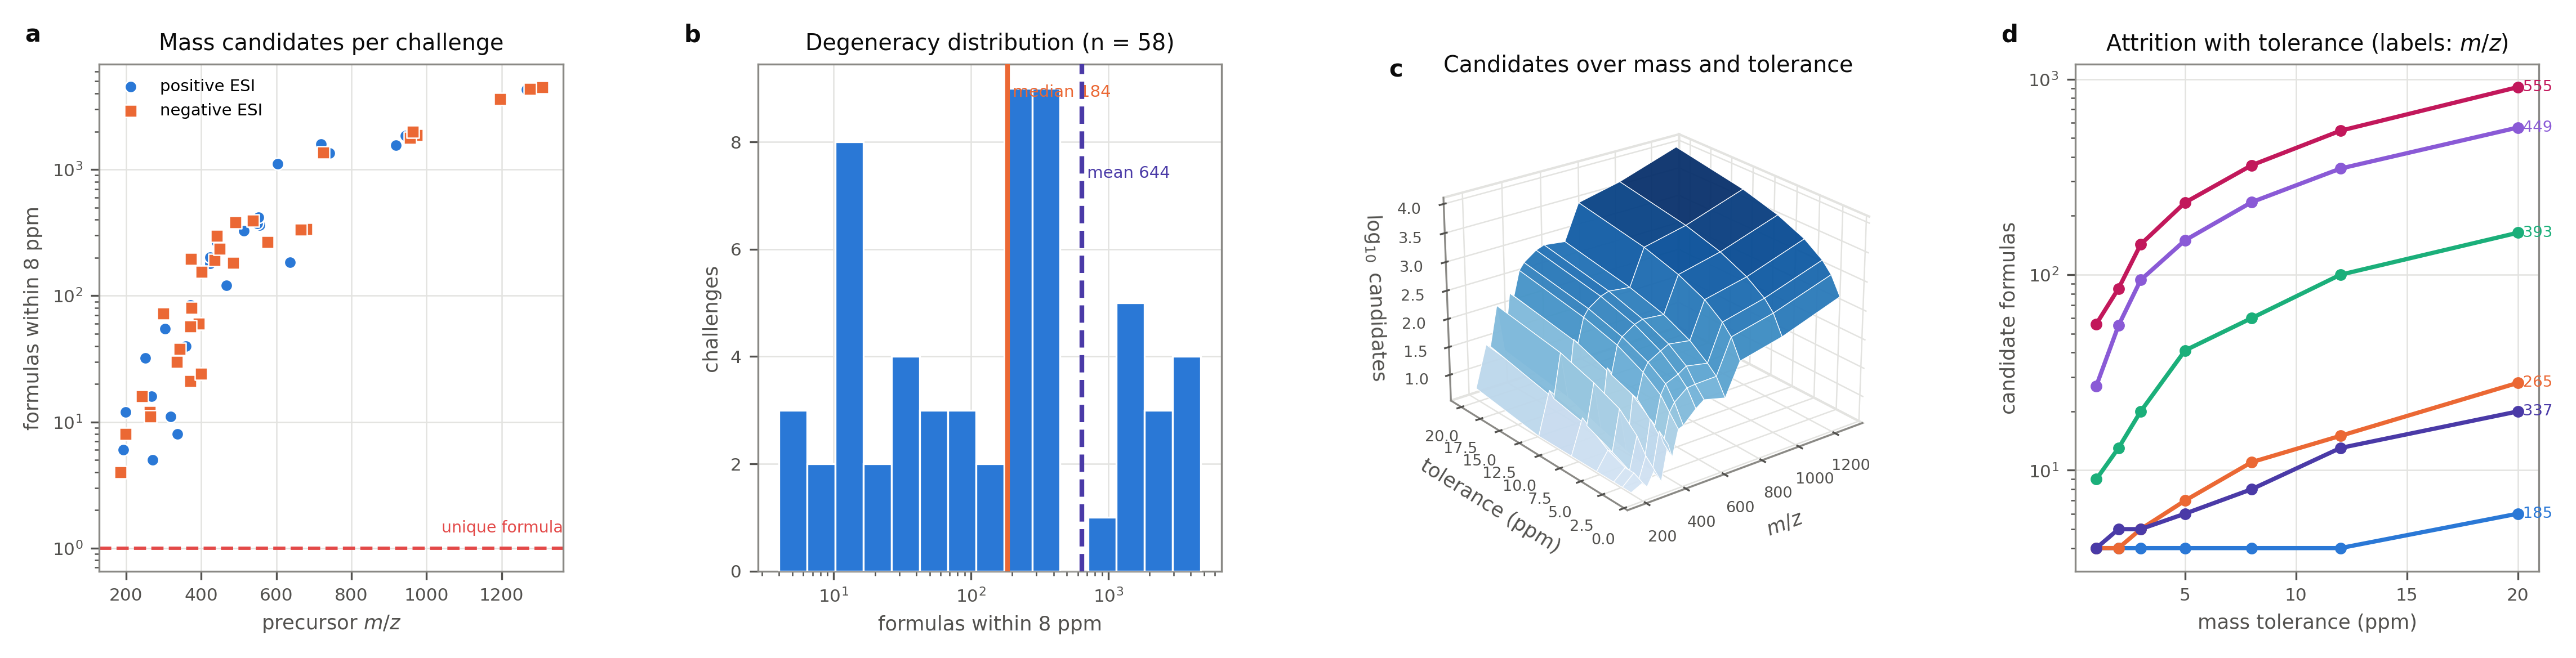
\includegraphics[width=\textwidth]{figures/panel1_degeneracy.png}
    \caption{\textbf{Exact mass does not determine formula: the degeneracy of the
    mass determination across 58 challenges.}
    (\textbf{A})~Uncapped count of distinct CHNOPS formulas satisfying the 8~ppm
    precursor window, plotted against precursor $m/z$ for all 58 challenges,
    separated by polarity. The count rises from 4 at the low-mass end to 4500 at
    the high-mass end; no challenge attains a count of one.
    (\textbf{B})~Distribution of the same counts on a logarithmic axis, with the
    median at 183 and the mean at 645; the singleton line at $|\Dmass| = 1$ is
    empty.
    (\textbf{C})~Three-dimensional surface of candidate count over precursor
    $m/z$ and mass tolerance from 1 to 20~ppm. Tightening the window below the
    instrument's achievable accuracy does not collapse the count to unity at any
    mass above the low-mass end.
    (\textbf{D})~Candidate count against tolerance for individual challenges
    spanning the mass range, showing the approximately linear dependence on
    tolerance against the superlinear dependence on mass.}
    \label{fig:panel1}
\end{figure*}

\begin{figure*}[!htbp]
    \centering
    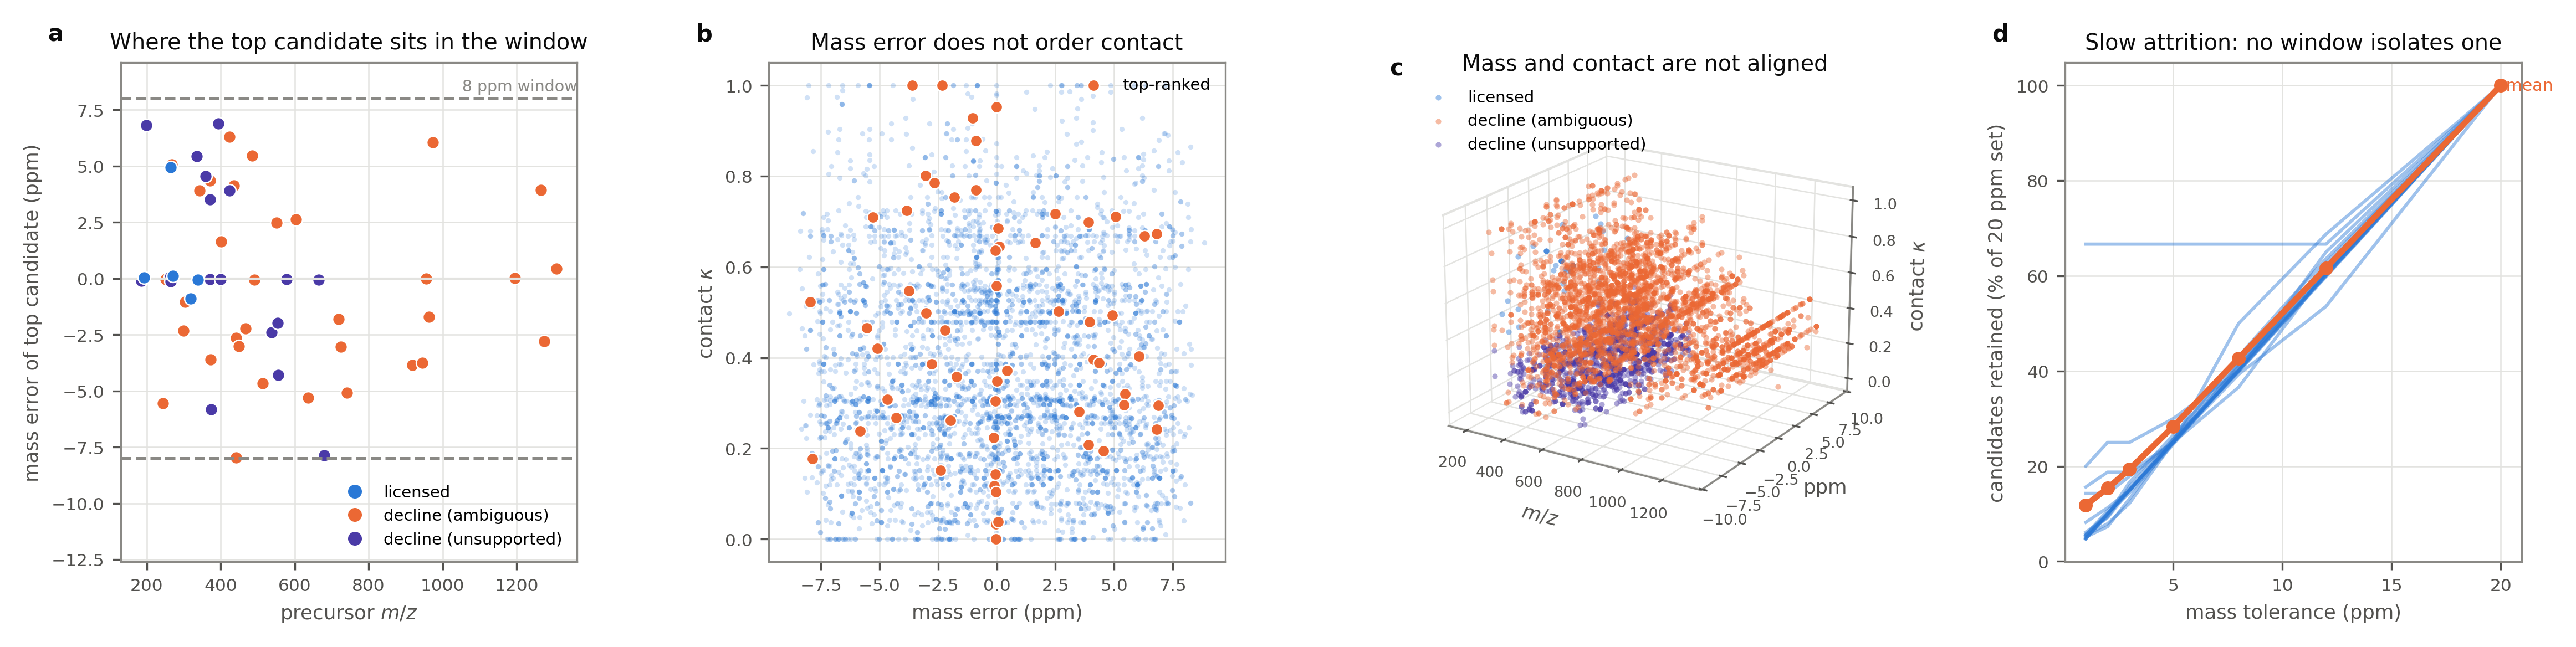
\includegraphics[width=\textwidth]{figures/panel2_tolerance.png}
    \caption{\textbf{Mass error, candidate density, and the geometry of the 8~ppm
    window.}
    (\textbf{A})~Measured precursor mass error of the top-ranked candidate for
    each challenge against precursor $m/z$, with the 8~ppm acceptance envelope.
    Licensed challenges cluster near zero error; the single licensed challenge at
    $+4.94$~ppm is visible at the envelope's edge.
    (\textbf{B})~Candidate count against mass error for all scored candidates,
    showing that mass error alone does not order the candidate set.
    (\textbf{C})~Three-dimensional scatter of precursor $m/z$, mass error, and
    contact for every scored candidate, coloured by verdict class. Contact varies
    over the full range at every mass error, which is the geometric statement
    that the two determinations are not aligned.
    (\textbf{D})~Cumulative fraction of candidates retained as the tolerance is
    tightened, per challenge, showing the slow attrition that motivates a second
    determination. The single stepped curve is challenge 33, the least degenerate
    in the set: it holds 4 candidates from 1 to 12~ppm and reaches 6 only at
    20~ppm, so its retention quantises rather than varying smoothly.}
    \label{fig:panel2}
\end{figure*}

\begin{figure*}[!htbp]
    \centering
    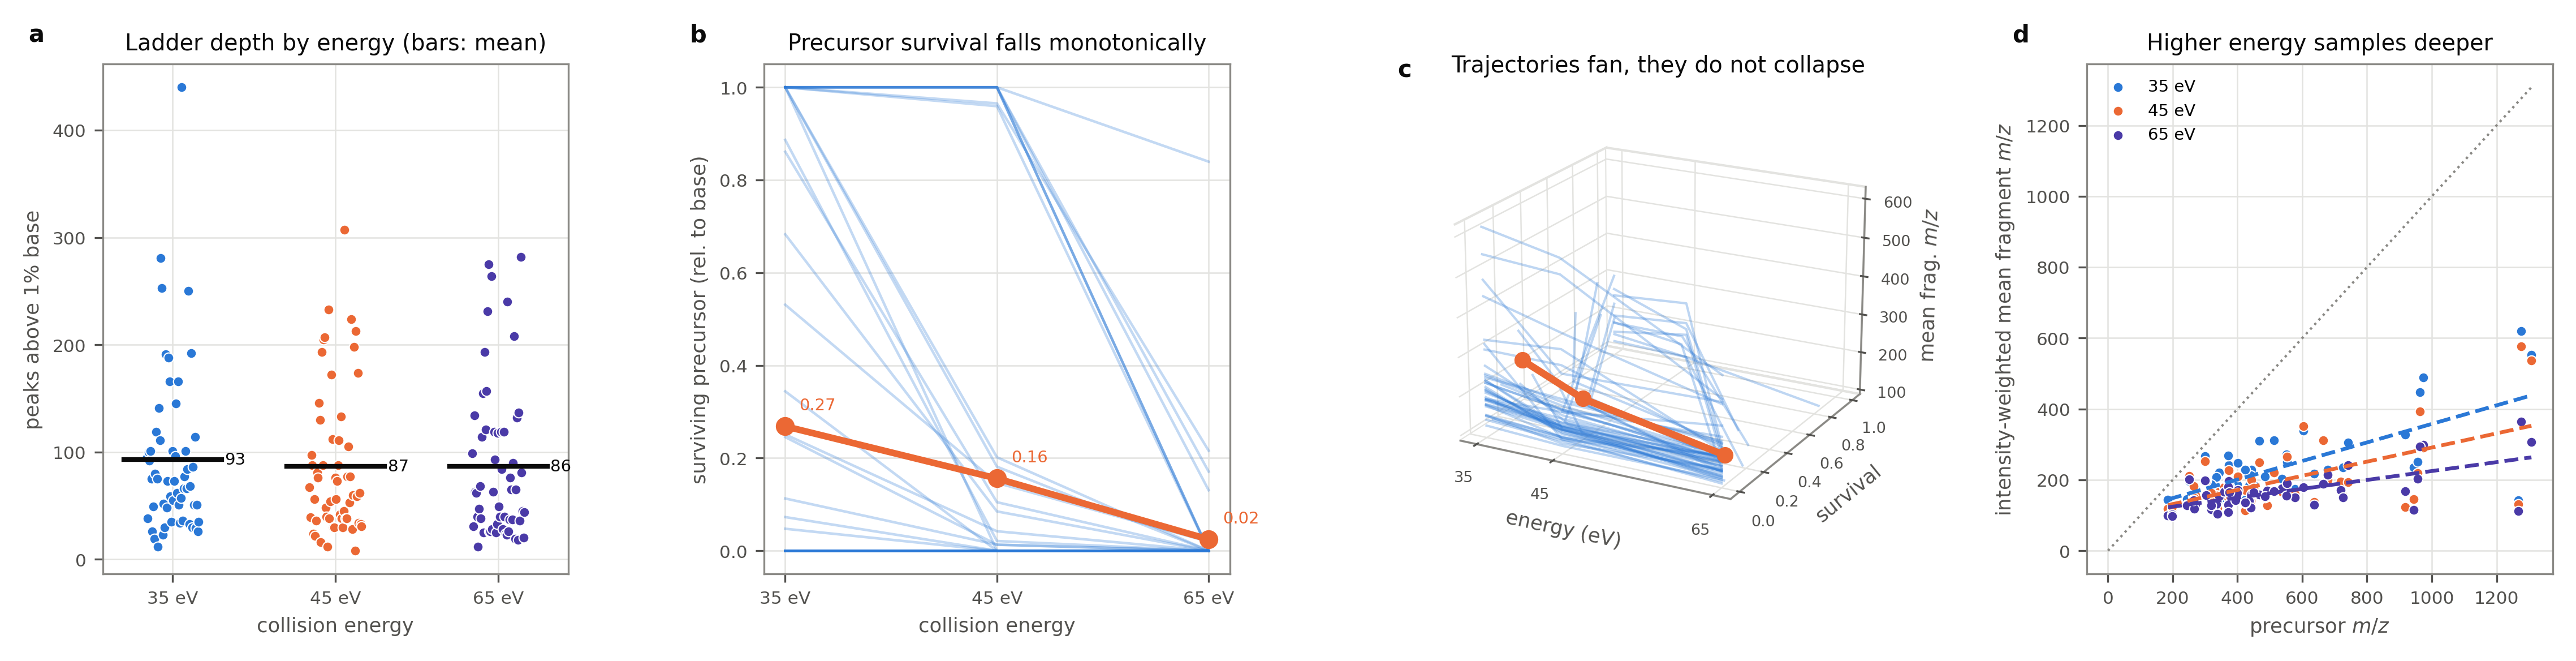
\includegraphics[width=\textwidth]{figures/panel3_energy.png}
    \caption{\textbf{The three collision energies are not redundant.}
    (\textbf{A})~Peak count per challenge at 35, 45 and 65~eV, paired by
    challenge, showing the ladder deepening and then thinning with energy.
    (\textbf{B})~Surviving precursor intensity, normalised to base peak, at each
    of the three energies. Survival falls monotonically with energy across the
    set.
    (\textbf{C})~Three-dimensional trajectory of each challenge through the space
    of collision energy, precursor survival, and intensity-weighted mean fragment
    $m/z$. The trajectories fan rather than collapse, which is why the energies
    are held as separate evidence channels rather than averaged.
    (\textbf{D})~Intensity-weighted mean fragment $m/z$ against precursor $m/z$
    at each energy, showing that higher energy samples deeper into the
    fragmentation cascade at every precursor mass.}
    \label{fig:panel3}
\end{figure*}

\begin{figure*}[!htbp]
    \centering
    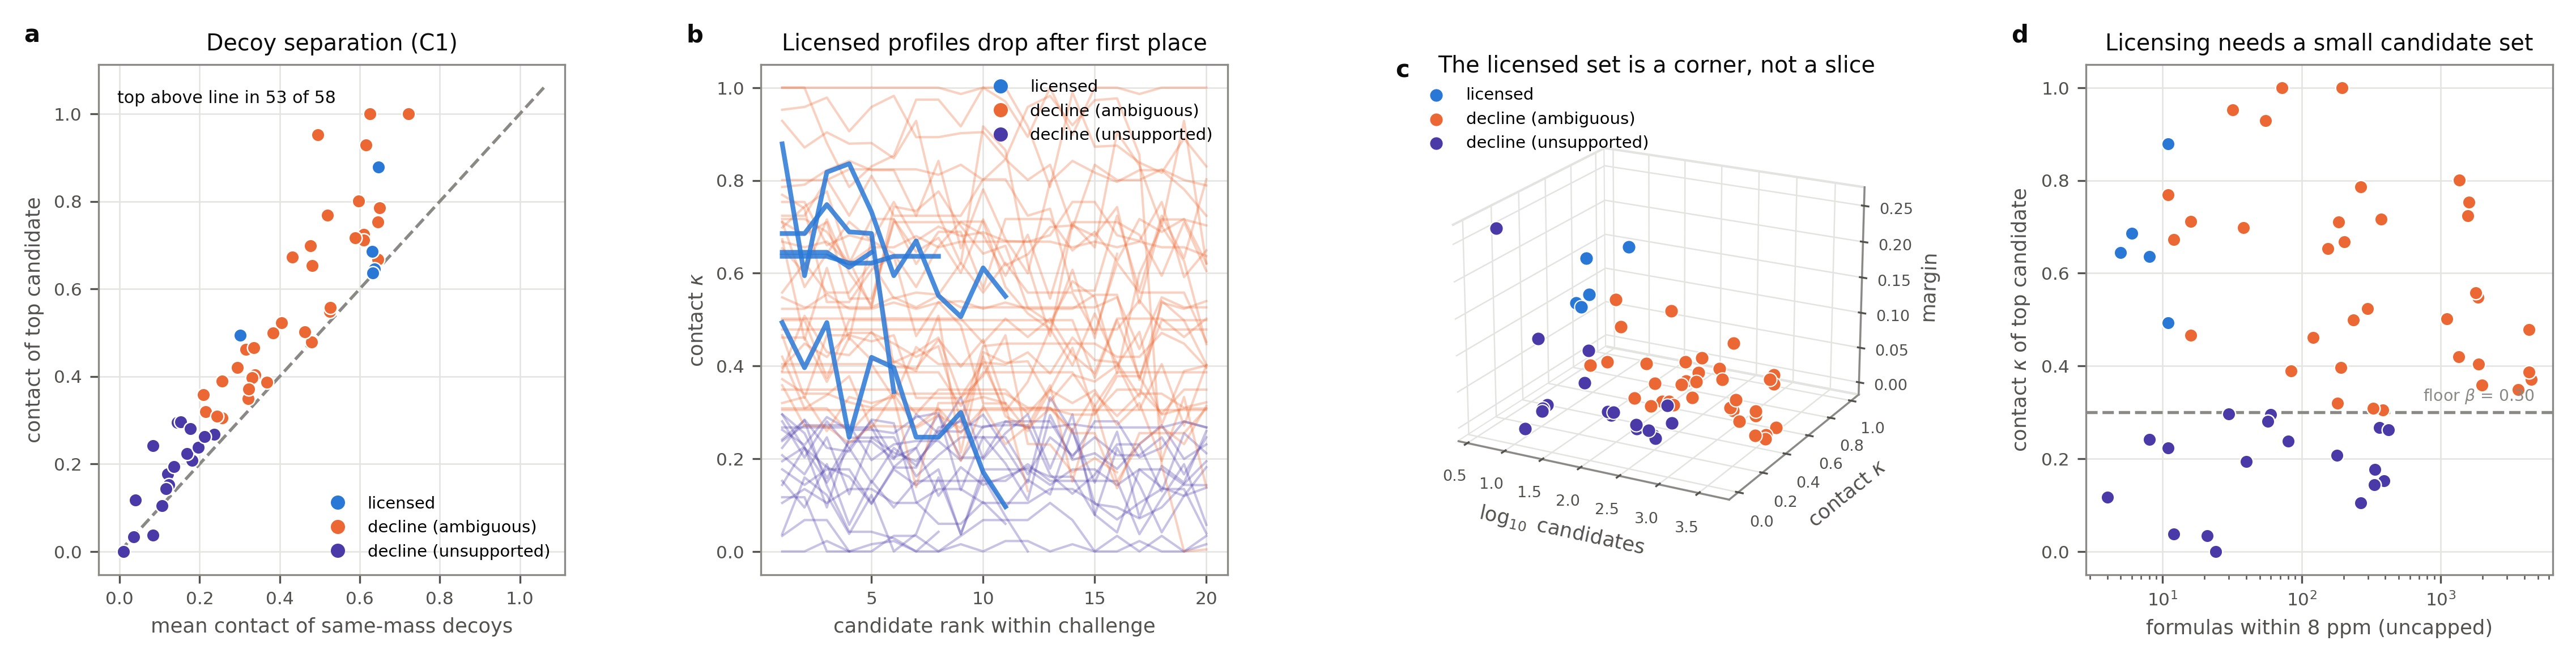
\includegraphics[width=\textwidth]{figures/panel4_contact.png}
    \caption{\textbf{Contact separates candidates that mass cannot.}
    (\textbf{A})~Contact of the top-ranked candidate against the mean contact of
    its same-mass decoys, one point per challenge, with the line of equality. The
    top candidate lies above the line in 53 of 58 challenges; mean separation
    $+0.1056$.
    (\textbf{B})~The ordered contact profile of the twenty highest-scoring
    candidates within each challenge, one curve per challenge, showing that in
    licensed cases the profile drops sharply after first place and in ambiguous
    cases it does not.
    (\textbf{C})~Three-dimensional scatter of mass degeneracy, contact, and
    margin for all 58 challenges, coloured by verdict. The licensed region is a
    corner of the space, not a slice through one axis.
    (\textbf{D})~Contact of the top candidate against uncapped mass degeneracy,
    showing that the licensed challenges are those where the candidate set was
    already small.}
    \label{fig:panel4}
\end{figure*}

\begin{figure*}[!htbp]
    \centering
    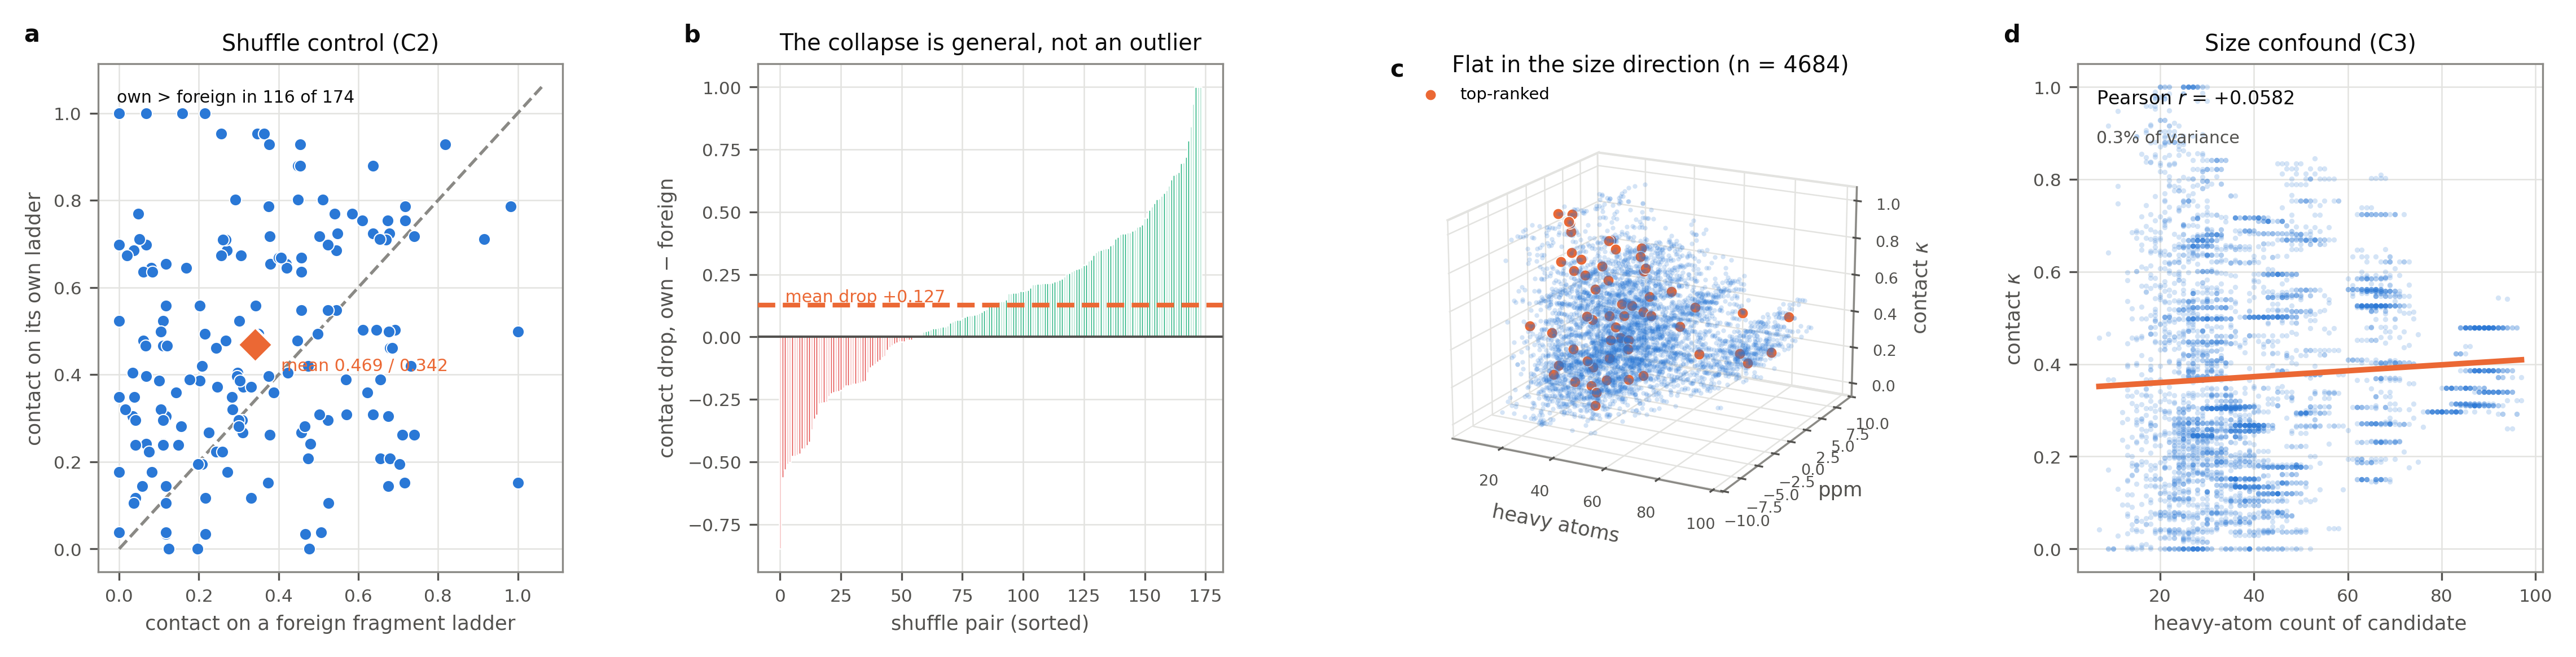
\includegraphics[width=\textwidth]{figures/panel5_controls.png}
    \caption{\textbf{Three controls: contact is structural, not size, and not
    coincidence.}
    (\textbf{A})~Shuffle control. Contact of each top candidate on its own
    fragment ladder against its contact on a foreign ladder of the same polarity,
    174 pairs, three per challenge. The mean falls from 0.469 to 0.342.
    (\textbf{B})~Paired drop per shuffle pair, sorted. The drop is positive in
    116 of 174 pairs and negative in the remaining 58: the effect is carried by a
    two-thirds majority, not by every pair and not by a few outliers.
    (\textbf{C})~Three-dimensional scatter of heavy-atom count, mass error, and
    contact over all 4684 scored candidate--fragment pairs. The cloud is flat in
    the size direction: Pearson $r = +0.0582$, so size explains 0.3\% of the
    variance in contact.
    (\textbf{D})~Contact against heavy-atom count with the fitted line, the
    direct visual form of the C3 correlation.}
    \label{fig:panel5}
\end{figure*}

\begin{figure*}[!htbp]
    \centering
    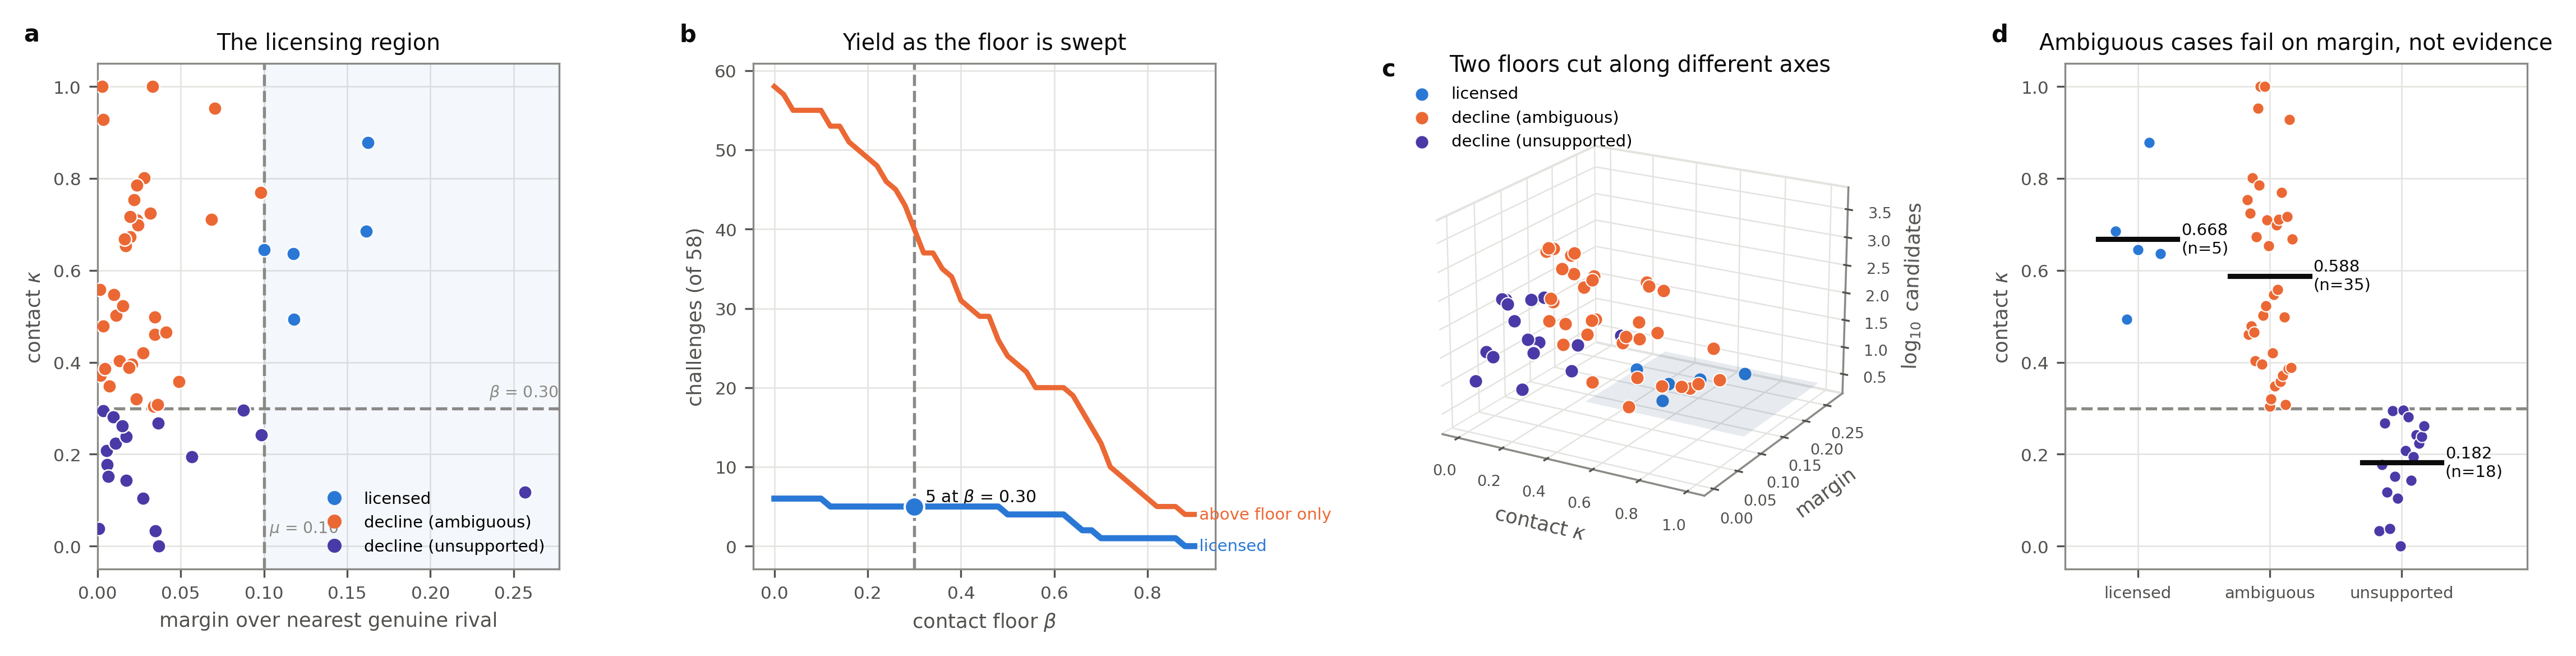
\includegraphics[width=\textwidth]{figures/panel6_licensing.png}
    \caption{\textbf{The floor, the decline, and what is bought by declining.}
    (\textbf{A})~Contact against margin for all 58 challenges with the licensing
    region $\con \ge 0.30$, margin $\ge 0.10$ marked. Five challenges fall inside
    it.
    (\textbf{B})~Licensed count as the contact floor $\beta$ is swept, showing
    the yield the method would report at every threshold and the cost of the one
    chosen.
    (\textbf{C})~Three-dimensional view of contact, margin, and mass degeneracy
    with the licensing region as a bounded volume, showing that the two floors
    cut the space along different axes and that neither alone isolates the
    licensed set.
    (\textbf{D})~Contact distribution by verdict class --- licensed 0.668,
    ambiguous 0.588, unsupported 0.182 --- showing that the ambiguous class fails
    on margin rather than on evidence.}
    \label{fig:panel6}
\end{figure*}

% =====================================================================
\section{Discussion}
% =====================================================================

\subsection{Against the single ranked list}

The dominant output format in metabolite identification is a ranked candidate
list~\citep{duhrkop2019sirius,ruttkies2016metfrag,blazenovic2018software}, often
with a score attached. A rank is a useful object, but it is not a determination,
and the difference is that a rank always exists. When two candidates are
separated by 0.30 in contact and when they are separated by 0.003, the ranked
list looks the same. Reporting the margin alongside the winner --- or, as here,
refusing to report a winner when the margin is small --- makes the difference
visible at the point of use.

The confidence-level frameworks that the field has
adopted~\citep{schymanski2014identifying,sumner2007proposed} are the right instinct
applied at the wrong granularity: they classify the \emph{kind} of evidence
available (library match, MS/MS, exact mass) rather than measuring, on this
spectrum, whether the evidence actually discriminated. A level-2 assignment and a
level-2 non-assignment are the same level.

\subsection{What a second determination has to satisfy}

The construction here generalises past this dataset. To be a second determination
rather than a second score, a quantity must (i) read a part of the measurement the
first determination does not, (ii) be shown to respond to that part rather than to
the candidate --- the shuffle control is the operational test --- and (iii) be
shown not to be a monotone function of some property of the candidate that would
make it a reparameterisation of the first. Contact satisfies all three here, but
so might isotope-pattern correspondence, retention-time prediction, or
collision-cross-section agreement, each of which reads a different channel. The
argument is for the structure, not for this particular instance of it.

\subsection{Why the yield is low, and what would raise it}

Five of 58 is a low yield and the reasons are visible in \Cref{tab:verdicts}. The
binding constraint is the margin, not the floor: 35 of the 53 declines had contact
above $\beta$ and failed only to separate. Their median degeneracy is 267. The
floor sweep makes this exact --- $\beta$ can be raised from 0.30 to 0.40 without
changing a single verdict (\Cref{sec:validation}) --- so $\beta$ is not the
constraint anywhere on this data. What
would raise the yield is therefore anything that shrinks $\Dmass$ before contact
is asked to do the separating --- isotope-pattern filtering, which the profile
data would support and which we did not implement; retention-time constraints from
the chromatography; or a database prior restricting composition to observed
biological space, at the cost of foreclosing the novel compounds CASMI exists to
test. Raising the yield by lowering $\mu$ would not shrink the candidate set; it
would only stop reporting that the candidate set is large.

\subsection{Limitations}

\begin{itemize}[leftmargin=1.4em]
\item \textbf{No grading.} See \Cref{sec:defect-key}. Nothing here is checked
against truth.
\item \textbf{Prior-carried margins.} See \Cref{sec:defect-prior}. One licensed
answer in five.
\item \textbf{Composition space.} CHNOPS plus Cl, Na, K in adducts only. A true
formula containing another halogen, a metal, or a heavier heteroatom is not in
$\Dmass$ and cannot be found by any amount of contact.
\item \textbf{Categories 3 and 4 not attempted.} The method determines
composition. Structure class and 2D structure require a structural model that this
construction does not contain.
\item \textbf{Subset, not the full contest.} 58 of 250 priority challenges, fixed
by which files were downloaded rather than by any property of the compounds, but a
subset nonetheless.
\item \textbf{Single dataset, single instrument.} The tolerances, the intensity
threshold, and the weighting of the three energies are calibrated to one Q~Exactive
HF method and have not been transferred.
\end{itemize}

% =====================================================================
\section{Conclusion}
% =====================================================================

Exact mass gives a unique elemental formula in none of the 58 CASMI challenges
recoverable from the data at hand; the median challenge admits 183 candidates and
the worst admits 4500. Fragment contact --- the intensity-weighted fraction of the
observed ladder a candidate explains as its own subformulas, measured across three
collision energies held as separate channels --- is a determination that reads a
disjoint part of the measurement and, by three controls, carries structural
information mass does not: it separates same-mass decoys in 53 of 58 cases, lowers
when scored on a foreign ladder, and correlates with candidate size at
$r = +0.058$.

Requiring the two determinations to agree, above an absolute floor and by a
margin, licenses 5 of 58 challenges and declines 53. We report that yield as the
result. A contest that grades a wrong answer and a blank identically creates an
incentive to answer regardless of evidence, and the honest response to that
incentive is to say, for each challenge, whether the measurement discriminated ---
and to accept the score that follows from saying so. Of the five answers we do
license, one has its margin carried by a chemical prior rather than by the
evidence, and we have said so rather than remove it quietly. None of the five is
graded, because the key was not available. What is established is narrower than an
identification and, we think, more durable: that a second determination exists, that
it is independent, and that its floor sorts the tractable challenges from the
intractable ones before any answer is committed.

% =====================================================================
\bibliographystyle{unsrtnat}
\bibliography{references}
% =====================================================================

\end{document}
